\documentclass{beamer}
\usefonttheme[onlymath]{serif}

\usepackage{braket}
\usepackage{tikz}

\usepackage{graphicx,amsmath, amssymb,color,url,booktabs,comment}  %cite
\urlstyle{sf}
%\usepackage[margin=1in]{geometry}
% \usepackage{fancyhdr}
%\usepackage[colorlinks]{hyperref} %pagebackref

\newcommand{\nc}{\newcommand}
\nc{\rnc}{\renewcommand}

\def\View{\mathsf{View}}

\def\GS{\mathsf{Ham}}
\nc{\cVGS}{\ensuremath{\cV_\GS}}

\def\Ver{\mathsf{Ver}}
\nc{\cVVer}{\ensuremath{\cV_\Ver}}

\def\Samp{\mathsf{Samp}}
\nc{\PiSamp}{\ensuremath{\Pi_\Samp}}
\nc{\VSamp}{\ensuremath{V_\Samp}}
\nc{\PSamp}{\ensuremath{P_\Samp}}
\nc{\PSampstar}{\ensuremath{P_\Samp^*}}
\nc{\cVSamp}[1]{\ensuremath{\cV_{\Samp,#1}}}
\nc{\cPSamp}[1]{\ensuremath{\cP_{\Samp,#1}}}

\def\SampZ{\mathsf{Final}}
\nc{\PiSampZ}{\ensuremath{\Pi_\SampZ}}
\nc{\VSampZ}{\ensuremath{V_\SampZ}}
\nc{\PSampZ}{\ensuremath{P_\SampZ}}
\nc{\PSampZstar}{\ensuremath{P_\SampZ^*}}
\nc{\cVSampZ}[1]{\ensuremath{\cV_{\SampZ,#1}}}
\nc{\cPSampZ}[1]{\ensuremath{\cP_{\SampZ,#1}}}

\def\HE{\mathsf{HE}}
\def\HGen{\mathsf{HE.Keygen}}
\def\HEnc{\mathsf{HE.Enc}}
\def\HEval{\mathsf{HE.Eval}}
\def\HDec{\mathsf{HE.Dec}}
\def\Rej{\mathsf{Rej}}

\def\QHE{\mathsf{QHE}}
\def\QGen{\mathsf{QHE.Keygen}}
\def\QEnc{\mathsf{QHE.Enc}}
\def\QEval{\mathsf{QHE.Eval}}
\def\QDec{\mathsf{QHE.Dec}}

\def\blind{\mathsf{blind}}
\nc{\Piblind}{\ensuremath{\Pi_\blind}}
\nc{\Vblind}{\ensuremath{V_\blind}}
\nc{\Pblind}{\ensuremath{P_\blind}}
\nc{\Pblindstar}{\ensuremath{P_\blind^*}}
\nc{\cVblind}[1]{\ensuremath{\cV_{\blind,#1}}}
\nc{\cPblind}[1]{\ensuremath{\cP_{\blind,#1}}}

\def\Pstar{P^*}
\nc{\cPstar}[1]{\ensuremath{\cP^*_{#1}}}
\nc{\ctx}[3]{\ensuremath{{{\widehat{#1}}_{#2}^{(#3)}}}}

\def\Measure{\mathsf{Measure}}
\nc{\PiMeasure}{\ensuremath{\Pi_\Measure}}
\nc{\VMeasure}{\ensuremath{V_\Measure}}
\nc{\PMeasure}{\ensuremath{P_\Measure}}
\nc{\PMeasureStar}{\ensuremath{P_\Measure^*}}
\nc{\cVMeasure}[1]{\ensuremath{\cV_{\Measure,#1}}}
\nc{\cPMeasure}[1]{\ensuremath{\cP_{\Measure,#1}}}

\def\Naive{\mathsf{int}}
\nc{\PiNaive}{\ensuremath{\Pi_\Naive}}
\nc{\VNaive}{\ensuremath{V_\Naive}}
\nc{\PNaive}{\ensuremath{P_\Naive}}
\nc{\PNaiveStar}{\ensuremath{P_\Naive^*}}
\nc{\cVNaive}[1]{\ensuremath{\cV_{\Naive,#1}}}
\nc{\cPNaive}[1]{\ensuremath{\cP_{\Naive,#1}}}
\nc{\cPNaiveStar}[1]{\ensuremath{\cP_{\Naive,#1}^*}}

\nc{\stepref}[1]{Step~\ref{step:#1}}

%
%\newcommand{\bra}[1]{\langle #1|}
%\newcommand{\ket}[1]{|#1\rangle}
\newcommand{\proj}[1]{|#1\rangle\langle #1|}
% \newcommand{\braket}[2]{\langle #1|#2\rangle}
% \newcommand{\Bra}[1]{\left\langle #1\right|}
% \newcommand{\Ket}[1]{\left|#1\right\rangle}
\newcommand{\Proj}[1]{\left|#1\right\rangle\left\langle #1\right|}
% \newcommand{\Braket}[2]{\left\langle #1\middle|#2\right\rangle}
\nc{\vev}[1]{\langle#1\rangle}
\nc{\grad}{{\vec{\nabla}}}
\nc{\abs}[1]{\lvert#1\rvert}
%\DeclareMathOperator{\abs}{abs}
\DeclareMathOperator{\Bin}{Bin}
\DeclareMathOperator{\conv}{conv}
\DeclareMathOperator{\eig}{eig}
\DeclareMathOperator{\Hist}{Hist}
\DeclareMathOperator{\Hyb}{Hyb}
\DeclareMathOperator{\id}{id}
\DeclareMathOperator{\Img}{Im}
\DeclareMathOperator{\Par}{Par}
\DeclareMathOperator{\poly}{poly}
\DeclareMathOperator{\negl}{negl}
\DeclareMathOperator{\polylog}{polylog}
\DeclareMathOperator{\tr}{tr}
\DeclareMathOperator{\rank}{rank}
% \DeclareMathOperator{\sgn}{sgn}
\DeclareMathOperator{\Sep}{Sep}
\DeclareMathOperator{\SepSym}{SepSym}
\DeclareMathOperator{\Span}{span}
\DeclareMathOperator{\supp}{supp}
\DeclareMathOperator{\swap}{SWAP}
\DeclareMathOperator{\Sym}{Sym}
\DeclareMathOperator{\ProdSym}{ProdSym}
\DeclareMathOperator{\SEP}{SEP}
\DeclareMathOperator{\PPT}{PPT}
\DeclareMathOperator{\Wg}{Wg}
\DeclareMathOperator{\WMEM}{WMEM}
\DeclareMathOperator{\WOPT}{WOPT}

\DeclareMathOperator{\BPP}{\mathsf{BPP}}
\DeclareMathOperator{\QPIP}{\mathsf{QPIP}}
\DeclareMathOperator{\SampBQP}{\mathsf{SampBQP}}
\DeclareMathOperator{\BQP}{\mathsf{BQP}}
\DeclareMathOperator{\FBQP}{\mathsf{FBQP}}
\DeclareMathOperator{\cnot}{\normalfont\textsc{cnot}}
\DeclareMathOperator{\DTIME}{\mathsf{DTIME}}
\DeclareMathOperator{\NTIME}{\mathsf{NTIME}}
\DeclareMathOperator{\MA}{\mathsf{MA}}
\DeclareMathOperator{\NP}{\mathsf{NP}}
\DeclareMathOperator{\NEXP}{\mathsf{NEXP}}
\DeclareMathOperator{\Ptime}{\mathsf{P}}
\DeclareMathOperator{\QMA}{\mathsf{QMA}}
\DeclareMathOperator{\QCMA}{\mathsf{QCMA}}
\DeclareMathOperator{\BellQMA}{\mathsf{BellQMA}}

\newcommand{\be}{\begin{equation}}
\newcommand{\ee}{\end{equation}}
\newcommand{\bea}{\begin{eqnarray}}
\newcommand{\eea}{\end{eqnarray}}
\newcommand{\nn}{\nonumber}
\newcommand{\bi}{\begin{itemize}}
\newcommand{\ei}{\end{itemize}}
\newcommand{\bn}{\begin{enumerate}}
\newcommand{\en}{\end{enumerate}}
\def\beas#1\eeas{\begin{eqnarray*}#1\end{eqnarray*}}
\def\ba#1\ea{\begin{align}#1\end{align}}
\nc{\bas}{\[\begin{aligned}}
\nc{\eas}{\end{aligned}\]}
\nc{\bpm}{\begin{pmatrix}}
\nc{\epm}{\end{pmatrix}}
\def\non{\nonumber}
\def\nn{\nonumber}
\def\eq#1{(\ref{eq:#1})}
\def\eqs#1#2{(\ref{eq:#1}) and (\ref{eq:#2})}
%\def\eq#1{Eq.~(\ref{eq:#1})}
%\def\eqs#1#2{Eqs.~(\ref{eq:#1}) and (\ref{eq:#2})}
\def\L{\left} 
\def\R{\right}
\def\ra{\rightarrow}
\def\ot{\otimes}
\nc{\given}{\ensuremath{\;\middle|\;}}

\iffalse

\newtheorem{theorem}{Theorem}[section]
\newenvironment{thm}{\begin{theorem}}{\end{theorem}}
%\newtheorem*{thm*}{Theorem}
%\newtheorem{claim}[thm]{Claim}
\newtheorem{cor}{Corollary}[theorem]
%\newtheorem{lem}{Lemma}[section]
\newtheorem{lemma}{Lemma}[section]
\newenvironment{lem}{\begin{lemma}}{\end{lemma}}
\newtheorem{remark}{Remark}[section]
\newenvironment{rmk}{\begin{remark}}{\end{remark}}
%\newtheorem{prop}[thm]{Proposition}
\newtheorem{definition}{Definition}[section]
\newenvironment{dfn}{\begin{definition}}{\end{definition}}
\newtheorem{fact}{Fact}[section]
%\newtheorem{con}[thm]{Conjecture}

\newenvironment{prf}{\begin{proof}}{\end{proof}}

\fi

\def\eps{\epsilon}
\def\va{{\vec{a}}}
\def\vb{{\vec{b}}}
\def\vn{{\vec{n}}}
\def\cvs{{\cdot\vec{\sigma}}}
\def\vx{{\vec{x}}}
\def\Usch{U_{\text{Sch}}}

\def\cA{\mathcal{A}}
\def\cB{\mathcal{B}}
\def\cD{\mathcal{D}}
\def\cE{\mathcal{E}}
\def\cF{\mathcal{F}}
\def\cH{\mathcal{H}}
\def\cI{{\cal I}}
\def\cL{{\cal L}}
\def\cM{{\cal M}}
\def\cN{\mathcal{N}}
\def\cO{{\cal O}}
\def\cP{\mathcal{P}}
\def\cQ{\mathcal{Q}}
\def\cS{\mathcal{S}}
\def\cT{{\cal T}}
\def\cU{\mathcal{U}}
\def\cV{\mathcal{V}}
\def\cW{{\cal W}}
\def\cX{{\cal X}}
\def\cY{{\cal Y}}

\def\bp{\mathbf{p}}
\def\bq{\mathbf{q}}
\def\bP{{\bf P}}
\def\bQ{{\bf Q}}
\def\gl{\mathfrak{gl}}

\def\bbC{\mathbb{C}}
% \DeclareMathOperator*{\E}{\mathbb{E}}
\DeclareMathOperator*{\bbE}{\mathbb{E}}
%\DeclareMathOperator*{\Pr}{Pr}
\nc{\Prob}[1]{\ensuremath{\Pr\left[#1\right]}}
\def\bbM{\mathbb{M}}
\def\bbN{\mathbb{N}}
\def\bbR{\mathbb{R}}
\def\bbZ{\mathbb{Z}}
\def\bbP{\mathbb{P}}
\def\bbV{\mathbb{V}}
\newcommand{\Real}{\textrm{Re}}

\def\benum{\begin{enumerate}}
\def\eenum{\end{enumerate}}
% \def\bit{\begin{itemize}}
% \def\eit{\end{itemize}}
\def\bdesc{\begin{description}}
\def\edesc{\end{description}}
\newcommand{\fig}[1]{Fig.~\ref{fig:#1}}
\newcommand{\tab}[1]{Table~\ref{tab:#1}}
\newcommand{\secref}[1]{Section~\ref{sec:#1}}
\newcommand{\appref}[1]{Appendix~\ref{sec:#1}}
\newcommand{\lemref}[1]{Lemma~\ref{lem:#1}}
\newcommand{\thmref}[1]{Theorem~\ref{thm:#1}}
\newcommand{\propref}[1]{Proposition~\ref{prop:#1}}
\newcommand{\protoref}[1]{Protocol~\ref{proto:#1}}
\nc{\myprotoref}[1]{\hyperref[#1]{Protocol~\ref*{#1}}}
\newcommand{\defref}[1]{Definition~\ref{def:#1}}
\newcommand{\corref}[1]{Corollary~\ref{cor:#1}}
\newcommand{\conref}[1]{Conjecture~\ref{con:#1}}

\newcommand{\FIXME}[1]{{\color{red}FIXME: #1}}
\nc{\todo}[1]{\textcolor{red}{todo: #1}}



\newcommand{\boxdfn}[2]{
\begin{figure}[h]
\begin{center}
\noindent \framebox{
\begin{minipage}{0.8\textwidth}
\begin{dfn}[{\bf #1}]
\ \\ \\
#2
\end{dfn}
\end{minipage}
}
\end{center}
\end{figure}
}

\newcommand{\boxproto}[2]{
\begin{figure}[h]
\begin{center}
\noindent \framebox{
\begin{minipage}{0.8\textwidth}
\begin{proto}[{\bf #1}]
\ \\ \\
#2
\end{proto}
\end{minipage}
}
\end{center}
\end{figure}
}

\def\begsub#1#2\endsub{\begin{subequations}\label{eq:#1}\begin{align}#2\end{align}\end{subequations}}
\nc\qand{\qquad\text{and}\qquad}
\nc\mnb[1]{\medskip\noindent{\bf #1}}
\nc\mn{\medskip\noindent}

\renewcommand{\arraystretch}{1.5}
%\nc{\problem}[1]{\item\noindent {\bf #1}}

\setlength{\tabcolsep}{10pt}

%%%%%% Han-Hsuan's commands %%%%%%%%
\nc{\nl}{\nn \\ &=}  %new line
\nc{\nnl}{\nn \\ &}  %new new line
\nc{\fot}{\frac{1}{2}} %frac one two
\nc{\oo}[1]{\frac{1}{#1}} % one over
\newcommand{\ben}{\begin{enumerate}}
\newcommand{\een}{\end{enumerate}}
\nc{\mc}{\mathcal}
\nc{\beq}{\begin{equation}}
\nc{\eeq}{\end{equation}}
% \nc{\norm}[1]{\L\| #1 \R\|}

\nc{\onenorm}[1]{\L\| #1 \R\|_1} %one norm
%\nc{\span}{\ensuremath{\mathrm{span}}}

\DeclareMathOperator*{\argmax}{arg\,max}

%\nc{1}

\newcommand{\hannote}[1]{\textcolor{blue}{\small {\textbf{(Han:} #1\textbf{) }}}}

\newcommand{\Knote}[1]{\textcolor{red}{\small {\textbf{(KM:} #1\textbf{) }}}}

\nc{\Ra}{\Rightarrow}
\nc{\zo}{\{0,1\}}	

%%%%import..
% \newcommand{\secpar}{n}


% %%%Efficient Verifier%
% \newcommand{\setupeff}{\setup_{\mathsf{eff}}}
% \newcommand{\vereff}{V_{\mathsf{eff}}}
% \newcommand{\vereffone}{V_{\mathsf{eff},1}}
% \newcommand{\vereffthree}{V_{\mathsf{eff},3}}
% \newcommand{\vereffout}{V_{\mathsf{eff},\mathsf{out}}}
% \newcommand{\proeff}{P_{\mathsf{eff}}}
% \newcommand{\proefftwo}{P_{\mathsf{eff},2}}
% \newcommand{\proefffour}{P_{\mathsf{eff},4}}
% \newcommand{\advPH}{{P^*}^{H}}
% \newcommand{\setup}{\mathsf{Setup}}
% \newcommand{\re}{\mathsf{re}}
% \newcommand{\crh}{\mathsf{CRH}}
% \newcommand{\transcript}{\mathsf{trans}}

% \newcommand{\setupefffs}{\setup_{\mathsf{eff}\text{-}\mathsf{fs}}}
% \newcommand{\proefffs}{P_{\mathsf{eff}\text{-}\mathsf{fs}}}
% \newcommand{\proefffstwo}{P_{\mathsf{eff}\text{-}\mathsf{fs},2}}
% \newcommand{\verefffs}{V_{\mathsf{eff}\text{-}\mathsf{fs}}}
% \newcommand{\verefffsone}{V_{\mathsf{eff}\text{-}\mathsf{fs},1}}
% \newcommand{\verefffsout}{V_{\mathsf{eff}\text{-}\mathsf{fs},\out}}
% %Games%
% \newcommand{\game}{\mathsf{Game}}

% %\newcommand*{\bra}[1]{\langle#1|}
% %\newcommand*{\ket}[1]{|#1\rangle}
% \newcommand*{\opro}[2]{|#1\rangle\langle#2|}
% \newcommand*{\ipro}[2]{\langle #1|#2\rangle}
% \newcommand{\TD}{\mathsf{TD}}

% %%%%% Registers %%%%%%%
% \newcommand*{\regK}{\mathbf{K}}
% \newcommand*{\regI}{\mathbf{I}}
% \newcommand*{\regR}{\mathbf{R}}
% \newcommand*{\regX}{\mathbf{X}}
% \newcommand*{\regY}{\mathbf{Y}}
% \newcommand*{\regZ}{\mathbf{Z}}
% \newcommand{\regW}{\mathbf{W}}
% \newcommand*{\regC}{\mathbf{C}}
% \newcommand*{\regO}{\mathbf{O}}
% \newcommand*{\regF}{\mathbf{F}}


\usetikzlibrary{shapes.callouts}
\usetikzlibrary{cd}
\usetheme{Copenhagen}

\title{Constant-round Blind Classical Verification of Quantum Sampling}

\begin{document}

\begin{frame}
	\titlepage
\end{frame}

\begin{frame}
	\frametitle{Settings}

	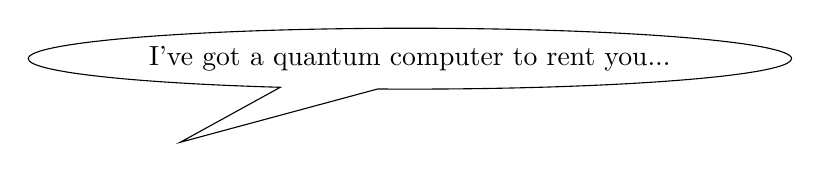
\begin{tikzpicture}
		\node[ellipse callout, callout relative pointer={(200:2cm)}, draw] (n1) {I've got a quantum computer to rent you...};
	\end{tikzpicture}

	\onslide<2->
	\begin{flushright}
		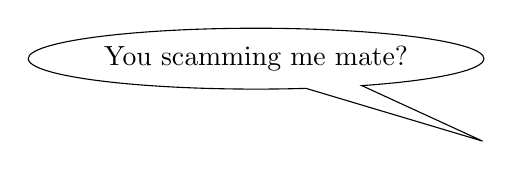
\begin{tikzpicture}
			\node[ellipse callout, callout relative pointer={(340:2cm)}, draw] (n2) {You scamming me mate?};
		\end{tikzpicture}
	\end{flushright}
\end{frame}

\begin{frame}
	\frametitle{Goal: $\BQP$? $\SampBQP$?}

    $\SampBQP$ is the class of sampling problems $\left(D_x\right)_{x\in\set{0, 1}^*}$ that can be (approximately) sampled by polynomial-size uniform quantum circuits. Namely, there exists a Turing machine $M$ such that for every $n \in \bbN$ and $\eps \in (0,1)$, $M(1^n, 1^{1/\eps})$ outputs a quantum circuit $C$ in $\poly(n, 1/\eps)$ time such that for every $x \in \zo^n$, the output of $C(x)$ (measured in standard basis) is $\eps$-close to $D_x$.

\end{frame}

\begin{frame}
	\frametitle{How might I get scammed?}
	\begin{itemize}[<+->]
		\item It doesn't even work! (correctness) (Solved for BQP)
		\item Stolen data (privacy)
	\end{itemize}
\end{frame}

\begin{frame}[fragile]
	\frametitle{Quantum Homomorphic Encryption Schemes}

	$$(pk, sk)\leftarrow\Gen(\lambda, 1^L)$$

	\begin{center}

		\begin{tikzcd}[row sep = 4.8em, column sep = 9.6em]
			X \rar["f(\,\cdot\,)"] \dar["{\Enc(pk, \,\cdot\,)}"] & Y \\
			\hat{X} \rar["{\Eval(pk, f, \,\cdot\,)}"] & \uar["{\Dec(sk, \,\cdot\,)}"] \hat{Y}
		\end{tikzcd}
	
	\end{center}

\end{frame}

\begin{frame}
	\frametitle{Compiler for blindness: Generic $\Pi=(P, V)(\lambda, x)$}
	\pause
	$(v_1, st_{V, 1})\leftarrow\cV_1(1^\lambda, x)$
	\pause
	\\\hspace*{\fill}$\xrightarrow{\qquad v_1\qquad}$\hspace*{\fill}
	\pause
	\\\hspace*{\fill}$(p_1, st_{P, 1})\leftarrow\cP_1(1^\lambda, v_1, x)$
	\pause
	\\\hspace*{\fill}$\xleftarrow{\qquad p_1\qquad}$\hspace*{\fill}
	\pause
	\\$(v_2, st_{V, 2})\leftarrow\cV_2(p_1, st_{V, 1})$
	\pause
	\\\hspace*{\fill}$\xrightarrow{\qquad v_2\qquad}$\hspace*{\fill}
	\pause
	\\\hspace*{\fill}$(p_2, st_{P, 2})\leftarrow\cP_2(v_1, st_{P, 1})$
	\pause
	\\\hspace*{\fill}$\xleftarrow{\qquad p_2\qquad}$\hspace*{\fill}
	\pause
	\\$(v_3, st_{V, 3})\leftarrow\cV_3(p_2, st_{V, 2})$
	\pause
	$$\vdots$$
	\pause
	$o\leftarrow\cV_{out}(p_T, st_{V,T})$
\end{frame}

\begin{frame}
	\frametitle{Compiler for blindness: Our $\Pi_\blind=(P_\blind, V_\blind(x))(\lambda)$}
	$(v_1, st_{V, 1})\leftarrow\cV_1(1^\lambda, x)$
	\pause
	\\$(pk_1, sk_1)\leftarrow\Gen(1^\lambda, 1^L)$
	\pause
	\\$\ctx{x}{}{1}\leftarrow\Enc(pk_1, x)$
	\pause
	\\$\ctx{v}{1}{1}\leftarrow\Enc(pk_1, v_1)$
	\pause
	\\\hspace*{\fill}$\xrightarrow{\qquad pk_1, \ctx{x}{}{1}, \ctx{v}{1}{1}\qquad}$\hspace*{\fill}
	\pause
	\\\hspace*{\fill}$\widehat{1^\lambda}\leftarrow\Enc(pk_1, 1^\lambda)$
	\pause
	\\\hspace*{\fill}$(\ctx{p}{1}{1}, \ctx{st}{P, 1}{1})\leftarrow\Eval(pk, \cP_1, \widehat{1^\lambda}, \ctx{v}{1}{1}, \ctx{x}{}{1})$
	\pause
	\\\hspace*{\fill}$\xleftarrow{\qquad \ctx{p}{1}{1}\qquad}$\hspace*{\fill}
	\pause
	\\$p_1\leftarrow\Dec(sk_1, \ctx{p}{1}{1})$
\end{frame}

\begin{frame}
	\frametitle{$\Pi_\blind=(P_\blind, V_\blind(x))(\lambda)$ cont.}
	$v_i\leftarrow\cV_2(p_{i-1}, st_{V, i-1})$

\end{frame}

\iffalse
        \item for $t=2,\ldots,T$:
        \begin{enumerate}
            \item $\Vblind$ decrypts the prover's last message by $p_{t-1}\leftarrow\QDec(sk_{t-1}, \ctx{p}{t-1}{t-1})$,
                then generates $(v_t, st_{V, t})\leftarrow\cV_t(p_{t-1}, st_{V, t-1})$.
                Then it generates $(pk_t, sk_t)\leftarrow\QGen(1^\lambda, 1^L)$,
                and produces encryptions $\ctx{v}{t}{t}\leftarrow\QEnc(pk_t, v_t)$ and $\ctx{sk}{t-1}{t}\leftarrow\QEnc(pk_t, sk_{t-1})$.
                It sends $pk_t$, $\ctx{v}{t}{t}$, and $\ctx{sk}{t-1}{t}$ to the prover.
            \item $\Pblind$ generates $(\ctx{p}{t}{t}, \ctx{st}{P, t}{t})\leftarrow\cPblind{t}(\ctx{v}{t}{t}, \ctx{sk}{t-1}{t}, \ctx{st}{P, t-1}{t-1})$
                by first switching its encryption key;
                that is, it encrypts its state under the new key by $\ctx{st}{P, t-1}{t-1, t}\leftarrow\QEnc(pk_t, \ctx{st}{P, t-1}{t-1}))$,
                then homomorphically decrypts the old encryption by
                $\ctx{st}{P, t-1}{t}\leftarrow\QEval(pk_t, \QDec,$ \ $\ctx{sk}{t-1}{t}, \ctx{st}{P, t-1}{t-1, t})$.
                Then it applies the next-message function homomorphically, generating
                $(\ctx{p}{t}{t}, \ctx{st}{P, t}{t})\leftarrow\QEval(pk_t, \cP_t, \ctx{v}{t}{t}, \ctx{st}{P, t-1}{t})$.
                It sends $\ctx{p}{t}{t}$ back to the verifier.
        \end{enumerate}
        \item $\Vblind$ decrypts the prover's final message by $p_T\leftarrow\QDec(sk_T, \ctx{p}{T}{T})$.
            It then computes its output $o\leftarrow\cV_{out}(p_T, st_{V, T})$.
\fi


\begin{frame}
	\frametitle{Compiler for blindness: Correctness}

\end{frame}

\begin{frame}
	\frametitle{Compiler for blindness: Blindness}

\end{frame}

\begin{frame}
	\frametitle{Verification under $\QPIP_1$ protocols}
	MF16 for BQP
	Different Hamiltonian for SampBQP

	Hcircuit and Hout
\end{frame}

\begin{frame}
	\frametitle{Mahadev's measurement protocol}

\end{frame}

\begin{frame}
	\frametitle{Parallel repetitions of measurement protocol?}

\end{frame}

\end{document}
